% !TEX root = ../main.tex
\subsubsection{DIS Cuts}
\label{sssec::dis_cuts}
    Three DIS cuts are applied to the scattered electron to restrict the phase space to that of Deep Inelastic Scattering (DIS).
    If the trigger electron fails to pass these cuts, all particles in the event are disregarded.

    The first cut is based on the invariant mass of the virtual photon, $Q^2$, and is defined as:
    \begin{equation*}
        Q^2 > 1 \text{ GeV}^2.
    \end{equation*}
    This ensures that the process falls within the DIS domain.

    The second cut is imposed on the squared mass of the hadronic final state, $W^2$, given by:
    \begin{equation*}
        W^2 > 4 \text{ GeV}^2.
    \end{equation*}
    Here, $W^2$ is defined as:
    \begin{equation*}
        W^2 = M^2 + 2M\nu - Q^2,
    \end{equation*}
    where $M$ represents the mass of the nucleon and $\nu$ is the energy fraction of the virtual photon.
    This cut is applied to exclude nucleon resonances.

    Lastly, an additional cut is imposed on the Bjorken-Y ($Y_b$) of the scattered electron, given by:
    \begin{equation*}
        Y_b < 0.85.
    \end{equation*}
    The Bjorken-Y ranges from 0 to 1 and is defined as:
    \begin{equation*}
        Y_b = \frac{\nu}{E_\text{beam}},
    \end{equation*}
    where $E_\text{beam}$ represents the energy of the incident electron beam.
    This cut effectively mitigates the influence of extreme radiative effects, which occur when a substantial portion of the incident electron's energy is transferred to the scattered electron.

    The impact of these cuts on the $Q^2$ and $\nu$ of the scattered electron can be observed in plot \ref{fig::q2vsnu}.

    \begin{figure}[b!]
        \centering\frame{
        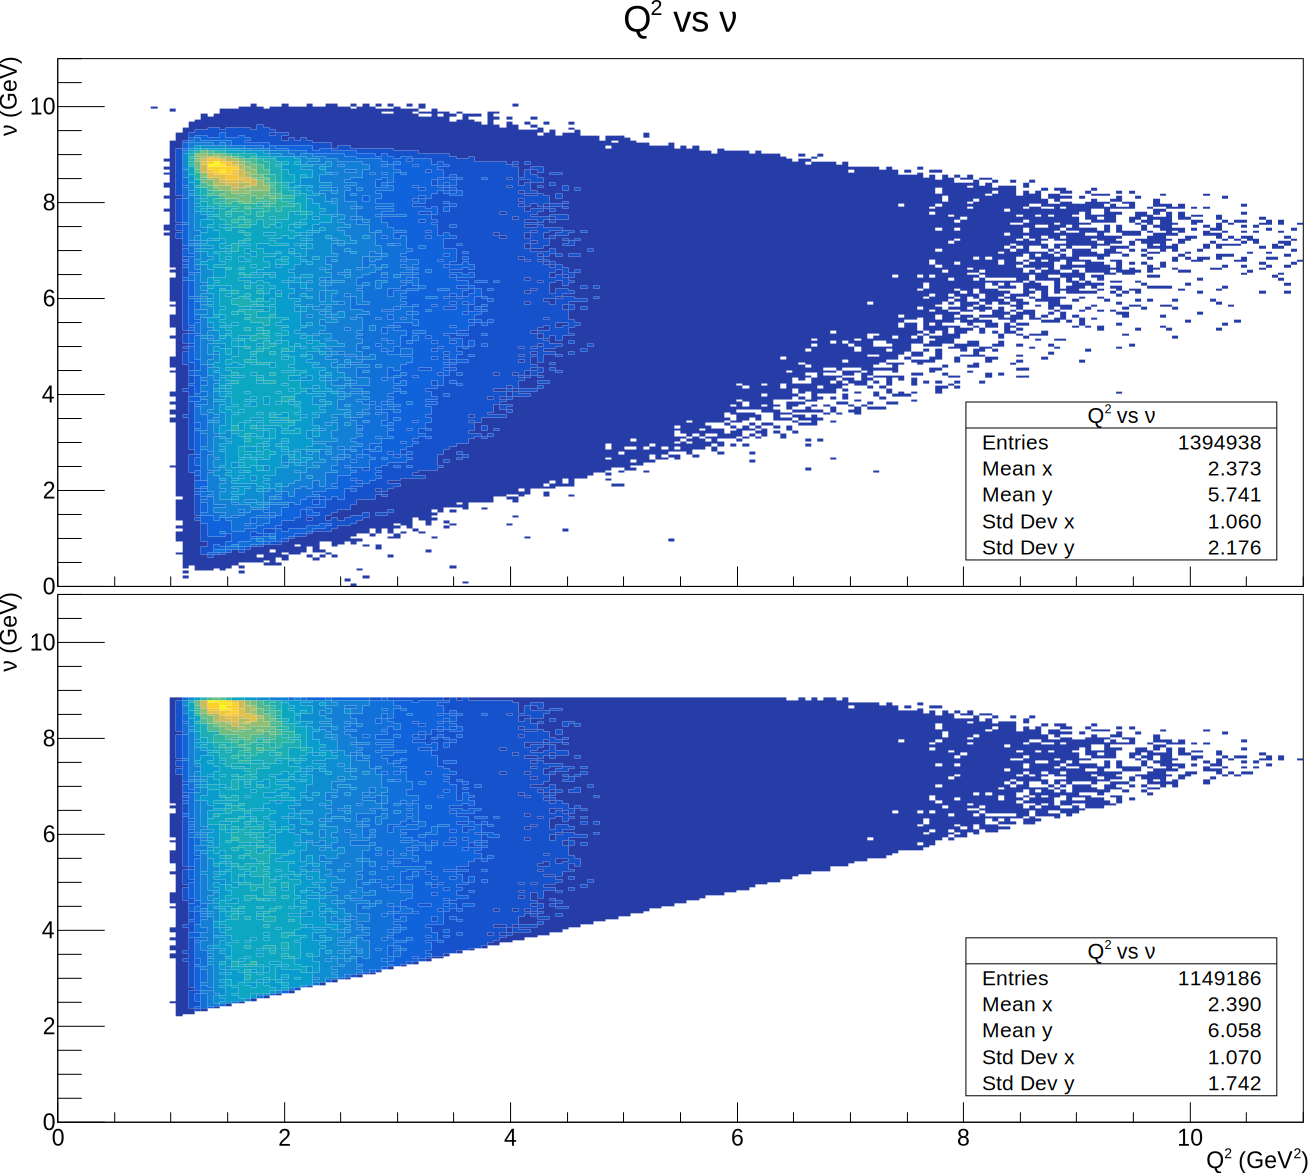
\includegraphics[width=\textwidth]{23q2_vs_nu.pdf}}
        \caption[$Q^2$ vs $\nu$ comparison]{$e^-$ $Q^2$ vs $\nu$ before and after applying the $Q^2 > 1 \text{ GeV}^2$, $W^2 > 4 \text{ GeV}^2$, and $Y_b < 0.85$ cuts, run 12016.
        Source: Own elaboration, using the \hyperlink{github.com/bleaktwig/clas12-rge-analysis}{clas12-rge-analysis} software.}
        \label{fig::q2vsnu}
    \end{figure}
